\begin{Ejc}
   Muestre que para $n-m>2$ se tiene que $$\int_{0}^{\infty}\frac{x^m}{x^n+1}=\frac{\pi}{n \phantom{o}\sen[\pi(m+1)/n]}.$$
\end{Ejc}
\begin{proof}
   Asumimos $m,n\in\mathbb{N}$. Llamemos $f(z)=z^m/(z^n+1)$ y $z_k=e^{\pi i (2k+1)/n}$ para $k\in{0,1,\dots,n-1}$; además, tomemos $\varphi=2\pi/n$ y $R>1$. Con lo anterior, llamamos $C_R$ a la curva $Re^{i\theta}$ con $\theta\in[0,\varphi]$, $C_1$ a la curva $re^{i\varphi}$ con $r$ variando de $R$ a $0$, y $C$ a la curva que consiste del eje real de $0$ a $R$, $C_R$ y $C_1$ (ver Figura 1).\\
%%%%%%%%%%%%%%%%%%%%%%%%%%%%%%%%%%%%%%%%%%%%
   %Imagen
   \begin{center}
       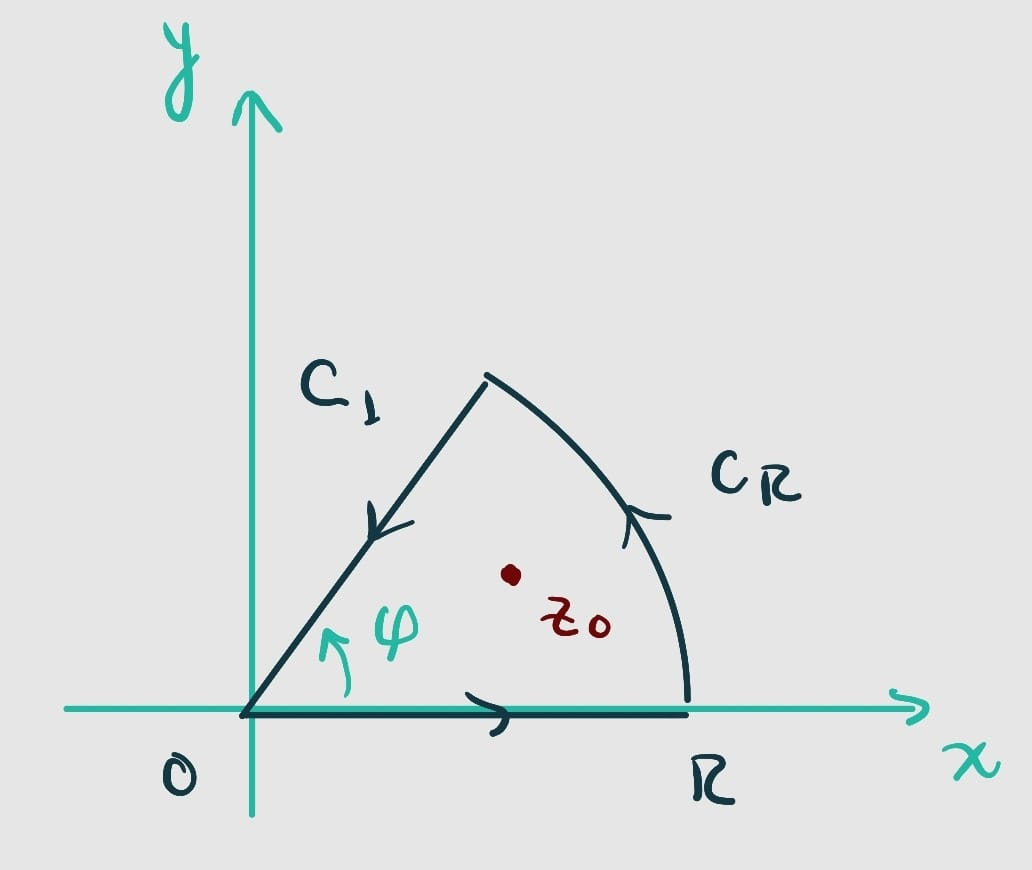
\includegraphics[height=3cm]{Diag1.jpeg}\\
       \captionof{Figura 1}
   \end{center}
%%%%%%%%%%%%%%%%%%%%%%%%%%%%%%%%%%%%%%%%%%%%
   Llamando
   $$
   \phi(z)=\frac{z^m}{\mathop{\prod\limits_{0<k\leq n-1}}(z-z_k)},
   $$
   tenemos $f(z)=\phi(z)/(z-z_0)$. Como $\phi(z)$ es analítica y no nula en $z_0$, entonces $z_0$ es un polo simple de $f(z)$ y
   $$
   \begin{aligned}
      B&:=\mathop{\mathrm{Res}}\limits_{z=z_0}f(z)\\
       &=\phi(z_0)\\
       &=\frac{{z_0}^m}{\mathop{\prod\limits_{0<k\leq n-1}}(z_0-z_k)}\\
       &=\frac{{z_0}^m}{\left.\left( \frac{z^n-1}{z-z_0}\right)\right|_{z=z_0}}.
   \end{aligned}
   $$
   Haciendo división sintética puede verse que
   $$
   \begin{aligned}
      \frac{z^n-1}{z-z_0}&=\sum_{k=1}^{n}{z_0}^{k-1}z^{n-k},
   \end{aligned}
   $$
   de modo que
   $$
   \begin{aligned}
      \left.\left( \frac{z^n-1}{z-z_0}\right)\right|_{z=z_0}&=\left.\left( \sum_{k=1}^{n}{z_0}^{k-1}z^{n-k}\right)\right|_{z=z_0}\\
                                                            &=\sum_{k=1}^{n}{z_0}^{k-1}{z_0}^{n-k}\\
                                                            &=\sum_{k=1}^{n}{z_0}^{n-1}\\
                                                            &=n{z_0}^{n-1},
   \end{aligned}
   $$
   y con esto
   $$
   \begin{aligned}
      B&=\frac{{z_0}^m}{n{z_0}^{n-1}}\\
       &=\frac{{z_0}^{m+1}}{n{z_0^n}}\\
       &=-\frac{{z_0}^{m+1}}{n}.
   \end{aligned}
   $$
   Como $z_0$ es el único cero de $z^n+1$ dentro de $C$, se tiene que $f(z)$ es analítica en $C$ y su interior salvo $z_0$. Por el teorema de los residuos de Cauchy obtenemos
   $$
   \int_{0}^{R}f(x)dx+\int_{C_R}f(z)dz+\int_{C_1}f(z)dz=\int_{C}f(z)dz=2\pi i B,
   $$
   o,
   $$
   \int_{0}^{R}f(x)dx+\int_{C_1}f(z)dz=2\pi i B-\int _{C_R}f(z)dz,
   $$
   Haciendo el cambio de variable $z=re^{i\varphi}$, $dz=e^{i\varphi} dr$ tenemos
   $$
   \begin{aligned}
      \int_{C_1}f(z)dz&=-\int_{0}^{R}f(re^{i\varphi})e^{i\varphi} dr\\
                      &=-e^{i\varphi}\int_{0}^{R}\frac{(re^{i\varphi})^m}{(re^{i\varphi})^n+1}dr\\
                      &=-e^{i\varphi}\int_{0}^{R}\frac{r^me^{im\varphi}}{r^ne^{in\varphi}+1}dr\\
                      &=-e^{i\varphi(m+1)}\int_{0}^{R}\frac{r^m}{r^n+1}dr\phantom{00000}(e^{in\varphi}=e^{in\frac{2\pi}{n}}=e^{i2\pi}=1)\\
                      &=-e^{i\varphi(m+1)}\int_{0}^{R}f(r)dr\\
                      &=-e^{i\varphi(m+1)}\int_{0}^{R}f(x)dx.
   \end{aligned}
   $$
   Así, de la igualdad
   $$
   \int_{0}^{R}f(x)dx+\int_{C_1}f(z)dz=2\pi i B-\int _{C_R}f(z)dz
   $$
   se sigue
   $$
   \begin{aligned}
      2\pi i B-\int_{C_R}f(z)dz&=\int_{0}^{R}f(x)dx-e^{i\varphi(m+1)}\int_0^{R}f(x)dx\\
                               &=\left( 1-e^{i\varphi(m+1)}\right)\int_{0}^{R}f(x)dx,
   \end{aligned}
   $$
   y, haciendo tender $R$ a $\infty$,
   $$
   \left( 1-e^{i\varphi(m+1)}\right)\int_{0}^{\infty}f(x)dx=2\pi i B-\lim_{R\to\infty}\int_{C_R}f(z)dz.
   $$
   Para cada $z\in C_R$ tenemos
   $$
   \begin{aligned}
      |z^n+1|&=|z^n-(-1)|\\
             &\geq||z^n|-|-1||\\
             &=|R^n-1|\\
             &=R^n-1,
   \end{aligned}
   $$
   donde en la última igualdad usamos que, como $R>1$ entonces $R^n>1$. Con lo anterior $1/|z^{n+1}|\leq 1/(R^n-1)$, de modo que
   $$
   \begin{aligned}
      |f(z)|&=\left|\frac{z^m}{z^n+1}\right|\\
            &=\frac{|z|^m}{|z^n+1|}\\
            &=\frac{R^m}{|z^n+1|}\\
            &\leq\frac{R^m}{R^n-1},
   \end{aligned}
   $$
   luego,
   $$
   \begin{aligned}
      \left|\int_{C_R}f(z)dz\right|&\leq \frac{R^m}{R^n-1}\varphi R\\
                                   &=\varphi \frac{R^{m+1}}{R^n-1}.
   \end{aligned}
   $$
   Como $n>m+2$, se tiene $\lim_{R\to\infty} \varphi R^{m+1}/(R^n-1)=0$, y con esto
   $$
   \lim_{R\to\infty}\int_{C_R}f(z)dz=0.
   $$
   Así,
   $$
   \left( 1-e^{i\varphi(m+1)}\right)\int_{0}^{\infty}f(x)dx=2\pi i B,
   $$
   es decir,
   $$
   \begin{aligned}
      \int_{0}^{\infty}f(x)dx&=\frac{2\pi i B}{1-e^{i\varphi(m+1)}}\\
                             &=-\frac{{z_0}^{m+1}}{n}\cdot\frac{2\pi i}{1-e^{i\varphi(m+1)}}\\
                             &=-\frac{{z_0}^{m+1}}{n}\cdot\frac{2\pi i}{1-\left( e^{i\varphi}\right)^{m+1}}.
   \end{aligned}
   $$
   Notemos que $e^{i\varphi}=e^{2\pi i/n}=\left( e^{\pi i/n}\right)^2={z_0}^2$, con lo que
   $$
   \begin{aligned}
      -\frac{{z_0}^{m+1}}{n}\cdot\frac{2\pi i}{1-\left( e^{i\varphi}\right)^{m+1}}&=-\frac{{z_0}^{m+1}}{n}\cdot\frac{2\pi i}{1-{z_0}^{2(m+1)}}\\
                                                                                  &=\frac{2\pi i}{n}\cdot\frac{1}{{z_0}^{m+1}-{z_0}^{-(m+1)}}.
   \end{aligned}
   $$
   Ahora, observemos que
   $$
   \begin{aligned}
      {z_0}^{m+1}-{z_0}^{-(m+1)}&=e^{\pi i(m+1)/n}-e^{-\pi i(m+1)/n}\\
                                &=e^{\pi i(m+1)/n}-\overline{e^{\pi i(m+1)/n}}\\
                                &=2i\cdot\text{Im}\left( e^{i\pi (m+1)/n}\right)\\
                                &=2i\cdot\sen[\pi(m+1)/n].
   \end{aligned}
   $$
   Con esto,
   $$
   \begin{aligned}
      \frac{2\pi i}{n}\cdot\frac{1}{{z_0}^{m+1}-{z_0}^{-(m+1)}}&=\frac{2\pi i}{n}\cdot\frac{1}{2i\cdot\sen[\pi(m+1)/n]}\\
                                                               &=\frac{\pi}{n\cdot\sen[\pi(m+1)/n]},
   \end{aligned}
   $$
   con lo que podemos concluir
   $$
   \int_{0}^{\infty}f(x)dx=\frac{\pi}{n\cdot\sen[\pi(m+1)/n]}.
   $$
\end{proof}
